%  LaTeX support: latex@mdpi.com 
%  For support, please attach all files needed for compiling as well as the log file, and specify your operating system, LaTeX version, and LaTeX editor.

%=================================================================
\documentclass[sport,article,submit,moreauthors,pdftex]{Definitions/mdpi} 
%=================================================================
% MDPI internal commands
\firstpage{1} 
\makeatletter 
\setcounter{page}{\@firstpage} 
\makeatother
\pubvolume{1}
\issuenum{1}
\articlenumber{0}
\pubyear{2021}
\copyrightyear{2021}
%\externaleditor{Academic Editor: Firstname Lastname} % For journal Automation, please change Academic Editor to "Communicated by"
\datereceived{} 
\dateaccepted{} 
\datepublished{} 
\hreflink{https://doi.org/} % If needed use \linebreak
%------------------------------------------------------------------
% The following line should be uncommented if the LaTeX file is uploaded to arXiv.org
%\pdfoutput=1

%=================================================================
% Add packages and commands here. The following packages are loaded in our class file: fontenc, inputenc, calc, indentfirst, fancyhdr, graphicx, epstopdf, lastpage, ifthen, lineno, float, amsmath, setspace, enumitem, mathpazo, booktabs, titlesec, etoolbox, tabto, xcolor, soul, multirow, microtype, tikz, totcount, changepage, paracol, attrib, upgreek, cleveref, amsthm, hyphenat, natbib, hyperref, footmisc, url, geometry, newfloat, caption
%=================================================================
% Full title of the paper (Capitalized)
\Title{Analysis of the kinematics of punches in karate and their recognition using an artificial neural network}

% MDPI internal command: Title for citation in the left column
\TitleCitation{Analysis of the kinematics of punches in karate and their recognition using an artificial neural network}

% Author Orchid ID: enter ID or remove command
%\newcommand{\orcidauthorA}{0000-0000-0000-000X} % Add \orcidA{} behind the author's name
%\newcommand{\orcidauthorB}{0000-0000-0000-000X} % Add \orcidB{} behind the author's name

% Authors, for the paper (add full first names)
\Author{Ilshat Khasanshin $^{1}$, Andrey Labintsev $^{2}$ and Dmitry Balashov $^{3}$}

% MDPI internal command: Authors, for metadata in PDF
\AuthorNames{Ilshat Khasanshin, Andrey Labintsev and Dmitry Balashov}

% MDPI internal command: Authors, for citation in the left column
\AuthorCitation{Khasanshin, I.; Labintsev, A.; Balashov, D.}
% If this is a Chicago style journal: Lastname, Firstname, Firstname Lastname, and Firstname Lastname.

% Affiliations / Addresses (Add [1] after \address if there is only one affiliation.)
\address{%
$^{1}$ \quad Financial University under the Government of the Russian Federation; iykhasanshin@fa.ru\\
$^{2}$ \quad Financial University under the Government of the Russian Federation; ailabintsev@fa.ru \\
$^{3}$ \quad Financial University under the Government of the Russian Federation; dabalashov@fa.ru }
\abstract{(1) Background: place the question addressed in a broad context and highlight the purpose of the study; (2) Methods: describe briefly the main methods or treatments applied; (3) Results: summarize the article's main findings; (4) Conclusion: indicate the main conclusions or interpretations. The abstract should be an objective representation of the article, it must not contain results which are not presented and substantiated in the main text and should not exaggerate the main conclusions.}
% Keywords
\keyword{punch; classification; sensors; neural networks (List three to ten pertinent keywords specific to the article; yet reasonably common within the subject discipline.)} 
\begin{document}
%%%%%%%%%%%%%%%%%%%%%%%%%%%%%%%%%%%%%%%%%%
\section{Introduction}
Karate is a traditional Japanese martial art. However, this Japanese martial art has gained popularity all over the world. Sports competitions of national and world level are held in karate. The popularity of karate as a sport is growing, and in this regard, the methods of training karate athletes are increasingly becoming scientific in nature.\\
To develop effective training techniques, trainers need to understand the kinematics and dynamics of karate punches. Therefore, our research was aimed to analyze the velocity fields of punches in karate, as well as to develop and analyze various models of artificial neural networks for recognizing punches.\\
To solve the problems of the study, inertial measurement units (IMUs) were used, which included an accelerometer and a gyroscope. IMUs were attached to the wrists of karate athletes. The use of IMUs was due to the fact that in sports and martial arts, they proved to be an effective tool for analyzing the kinematics and biomechanics of human movements \cite{ref-journal1, ref-journal2}.\\
In \cite{ref-journal3}, studies of the acceleration and speed of punches were carried out using IMUS that were installed on the wrists of boxers. The accelerometers in this study had a large range – 200g (g is the acceleration of gravity = 9.8 m / s2), but the acceleration graphs show that the maximum acceleration was about 25g. In addition, this acceleration corresponded to the final phase of the punch, when the athlete's fist stopped abruptly and this led to a large negative acceleration. This allows us to conclude that for studies of the kinematics of punches in martial arts, it is possible to limit the measurement range to 16-25g. In \cite{ref-journal3}, it was found that the speed of punches in male athletes was 8.1±1.4 m/s for jab-out punches, and 7.7 ± 1.5 m/s for cross-out punches. The women had the following results: 6.6 = 1.6 m / s (job-out), 5.7 = 1.5 m / s (cross-out).\\
The authors of the work \cite{ref-journal4} investigated the difference between the biomechanics of punches of elite and novice boxers based on IMUs, which in the amount of 17 pieces were installed on the body of boxers. IMUs had an accelerometer measurement limit of 18g, they included an accelerometer, gyroscope, magnetometer. Since the IMUs were installed on each body segment, the contribution of the body segments to the punching technique of boxers was determined. In both groups (elite and novice athletes), the elbow contributed the most to the cross-out technique, and the shoulder contributed the most to the hook and uppercut.\\
In \cite{ref-journal5}, the analysis of the kinematics of boxers ' punches using accelerometers was carried out in conjunction with videography. The authors [5] searched for the correlation of postures and fields of acceleration of blows with the fatigue of athletes. The graphs of punch accelerations given in [5] show that the maximum values are in the range of 20-40 m / s2, which also allows us to choose an IMU for experiments with a measurement limit of up to 16g. In [5], it is stated that a large number of degrees of freedom of human hands do not allow us to draw unambiguous conclusions about the kinematics of blows, so videography was additionally required. It can be noted that in this work, the magnetometer and gyroscope, which are usually included in the IMU, were not used, perhaps their use could lead to the fact that videography would not was needed.\\
Also, various techniques of artificial neural networks (ANN) are used to analyze the kinematics of punches in martial arts, which can also help in conditions of lack of data. The advantages of ANN have led to the fact that they are actively used in sports and martial arts \cite{ref-journal6}. For example, the authors \cite{ref-journal3} concluded that according to the accelerometer data, it is difficult to find the time when the boxer's hand begins to return after a punch. It can be assumed that the use of ANN methods can cope with this problem.\\
In \cite{ref-journal7}, the ANN in the form of a multilayer perceptron was developed for the purpose of automating the data collection of boxers ' punches. The input data for ANN was the IMU data that was attached to the boxers ' wrist. The accuracy of punch recognition ranged from 87.2 ± 5.4 \% to 95.33 ± 2.51\%.\\
In \cite{ref-journal8}, six different deep machine learning models for recognizing boxers ' punches were investigated. The IMUs were installed in two versions: (1 – the IMUs was attached to both wrists; 2 – the IMUs was attached to both wrists and the third thoracic vertebra). The accuracy of the impact prediction was: for version 1 – 0.90 ± 0.12, for version 2-0.87 ± 0.09. For version 1, the support vector machine (SVM) model worked best (accuracy = 0.96), version 2 – the multi-layer perceptron neural network (MLP-NN) model (accuracy = 0.98).\\
Not much work is devoted to the analysis of punches in karate based on IMUs and ANN. And so far, no research has been conducted on a specific karate punch, which is called uraken in Japanese (a punch is made from the inside out).
%%%%%%%%%%%%%%%%%%%%%%%%%%%%%%%%%%%%%%%%%%
\section{Materials and Methods}
\subsection{Participants}
One healthy participant (n=1), wight = 100 kg, height = 190 cm with experience in Karate took part in the study. Ethical approval was granted by the Human Research Ethics Commitee at Financial University at Government of the Russian Federation.

\subsection{Materials}
One 6DOF Inertial Measurement Unit (IMU) T-Wristband with properties (sampling rate 50 Hz, +- 16 g linear acceleration, +- 2000 deg/s gyroscope) was used in this study. T-wristband bracelet with 252x19x12 basic dimensions, 47x18x12 host dimension, 30 g weight with custom firmware used.

\begin{figure}[H]
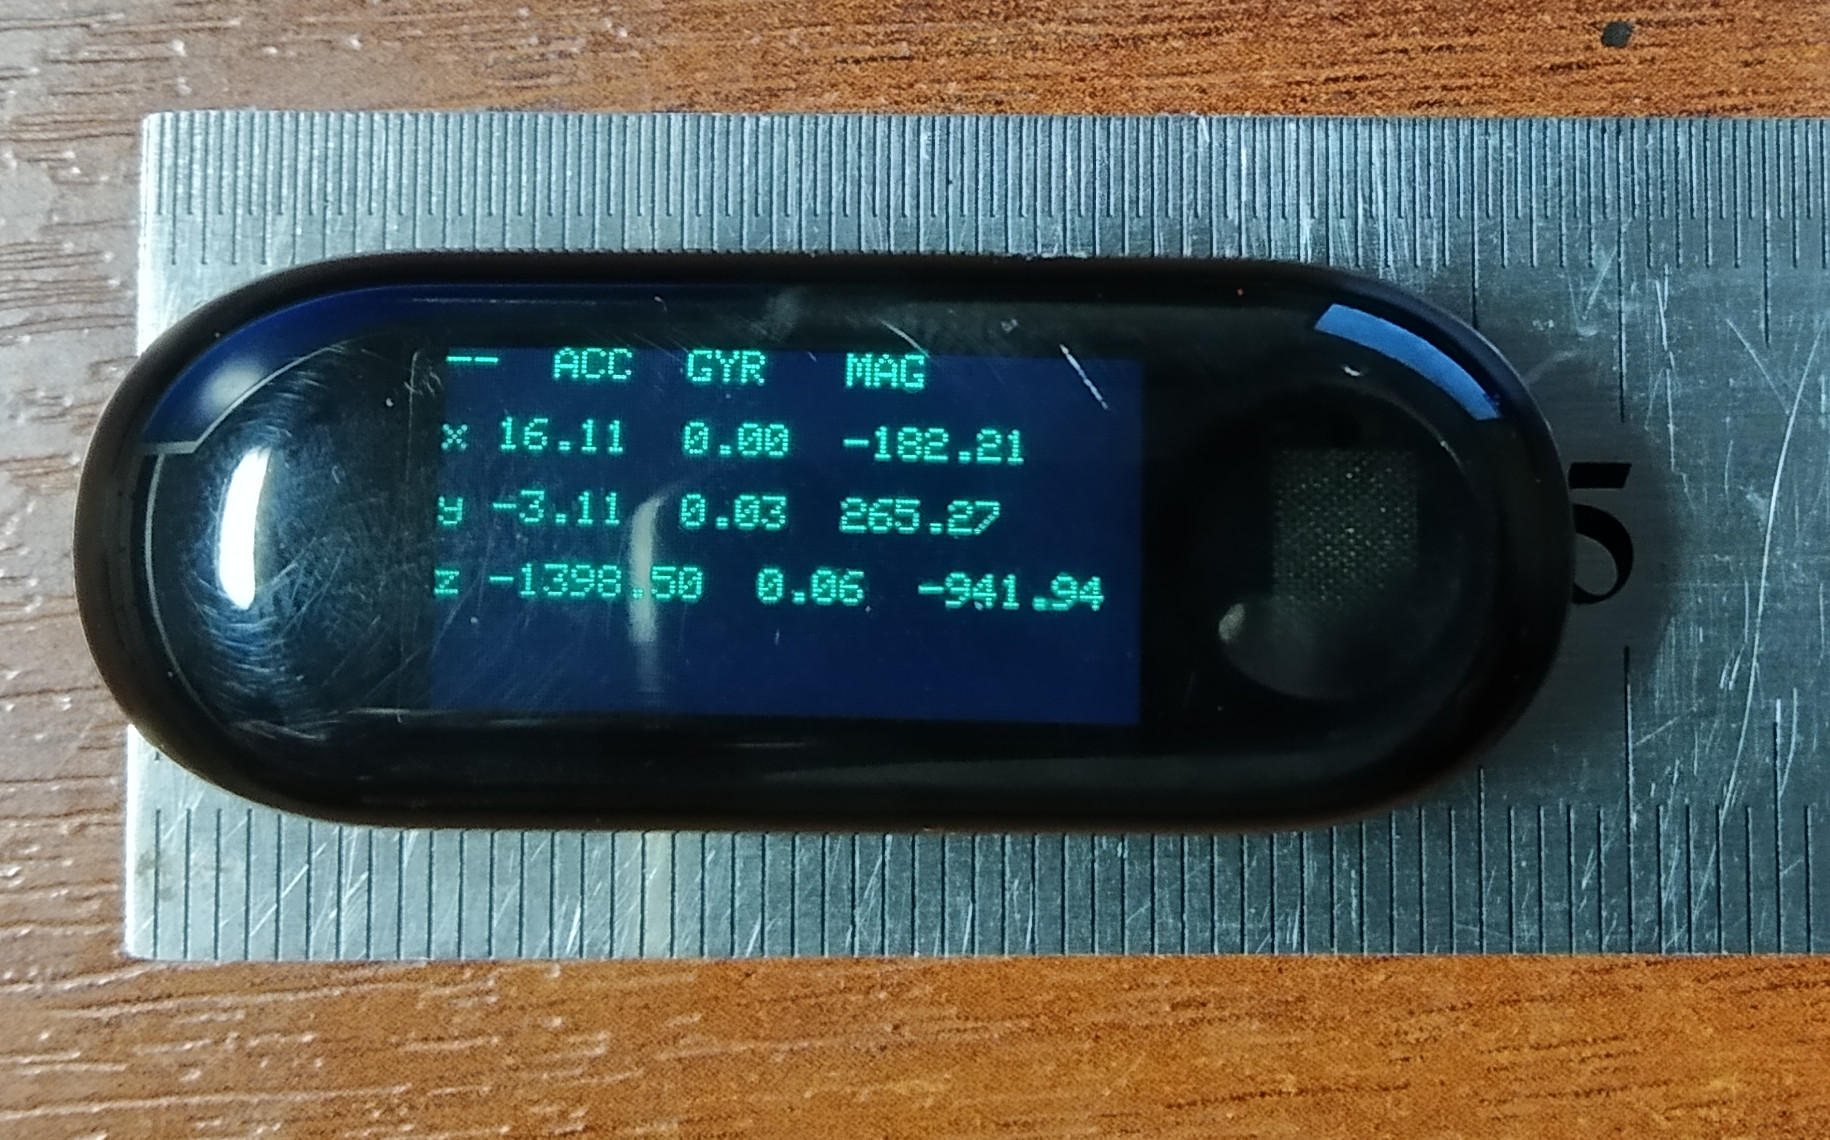
\includegraphics[width=10.5 cm]{img/IMU.jpg}
\caption{T-wristband size}
\end{figure} 

\begin{figure}[H]
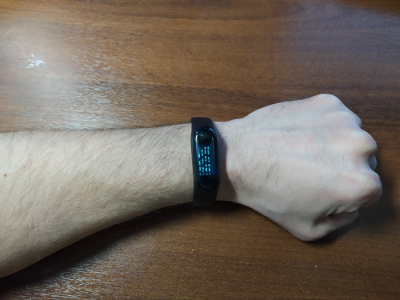
\includegraphics[width=10.5 cm]{img/hand_imu.jpg}
\caption{T-wristband host sensor was attached under on wrist}
\end{figure} 

We don't use magnitometer measurements and don't calculate angles and position of sensor. We use only linear acceleration and gyroscope measurements.

To record session we use Xiaomi Redmi 7 camera with 1980x1080 resolution 30 fps. Video analysis was used to labeling ground truth punches. To record data we use Bluetooth Serial Terminal Android application.

\subsection{Methods}
Data collection session consist of the participant performing 1912 punches to makivara.

Class of punches are:
\begin{enumerate}
\item	Yun Tsuki (YT); 
\item	Mawashi Tsuki (MT);
\item	Age Tsuki (AT);
\item	Uraken (U);
\item	No Punch (NP).
\end{enumerate}

\begin{figure}[H]
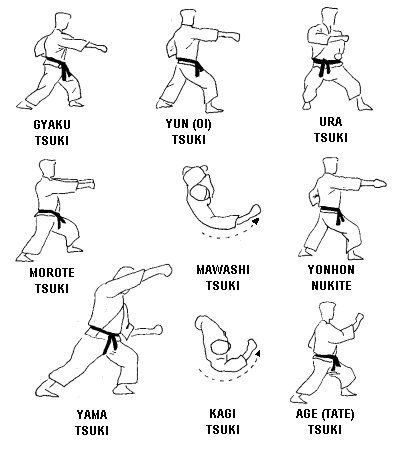
\includegraphics[width=10.5 cm]{img/punch_names.jpg}
\caption{Punch classes}
\end{figure} 

Measured data was packed to dataset X: every sample has 3 columns (x, y, z acceleration).

Train / validation random splitting was made with 10:1 propotional for each class.

\begin{figure}[H]
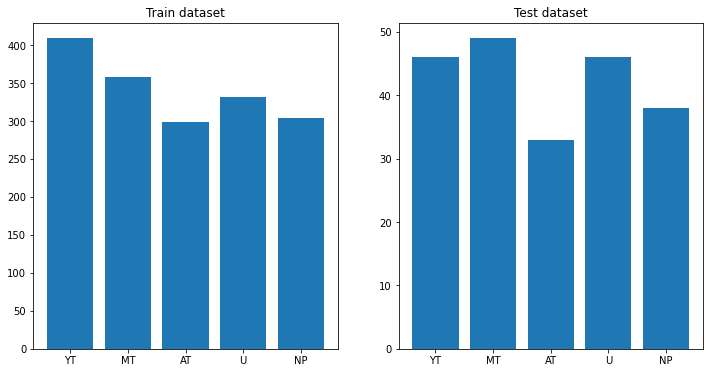
\includegraphics[width=10.5 cm]{img/train_test_data.png}
\caption{Train and test samples}
\end{figure} 

 Data preprocessing was conducted with python 3.7 packages: numpy, sklearn. Visualisation was made with matplotlib, Neural Net models build with tensorflow.keras 2.2.  
 
\begin{figure}[H]
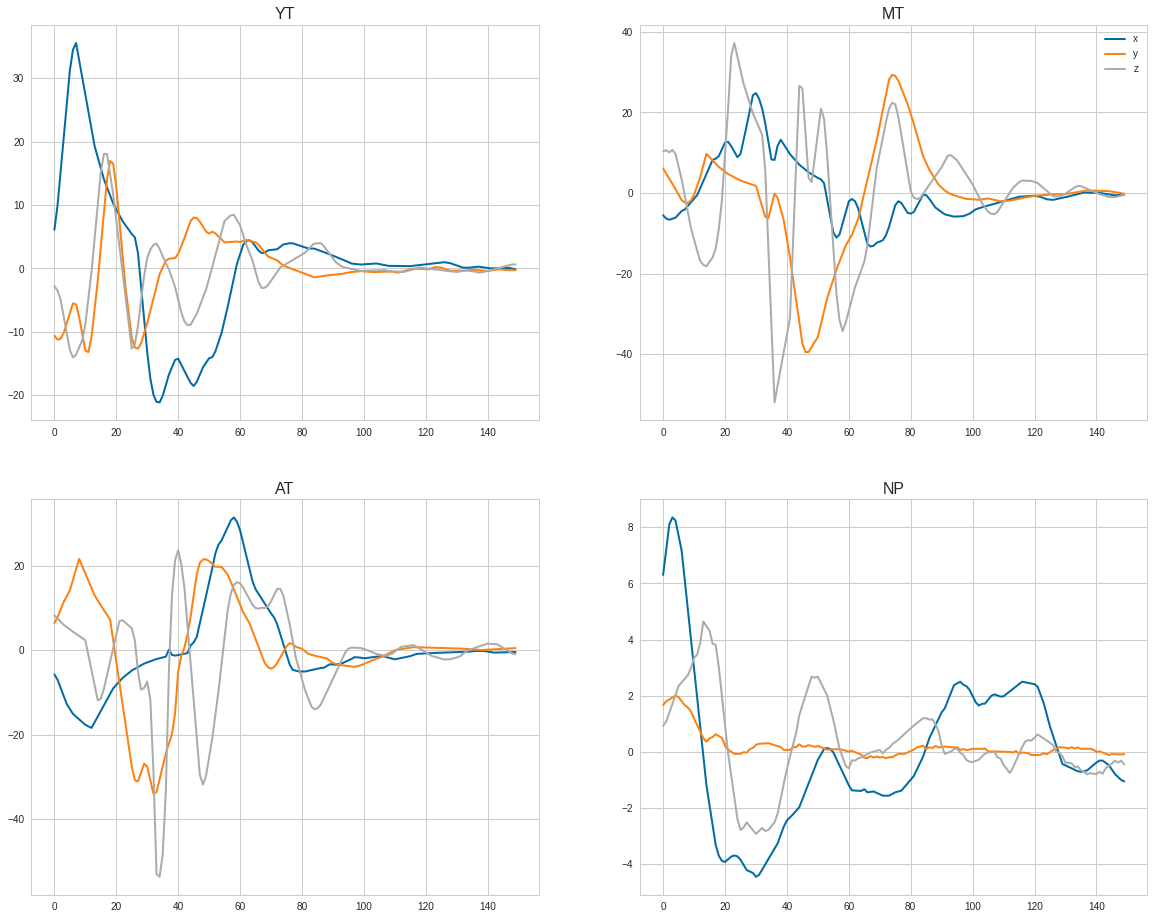
\includegraphics[width=10.5 cm]{img/data_xyz.png}
\caption{Measurement raw data visualized for different punch classes}
\end{figure} 

In experiments takes part 4 models:
\begin{enumerate}
\item	multylayer perceptron; 
\item	1 dimension convolution network from scratch;
\item	2 dimension convolution network with 2 layers;
\item	2 dimension convolution network with 4 layers.
\end{enumerate}

Multiclass Accuracy used as a classification metric for all classes:
\begin{equation}
ACC = \frac{N_T}{N}
\end{equation}

where $N_T$ - number of true classified punch,  
$N$ - total number of punches.\\
Precision, recall and F1-score were used as a classification metrics for single classes:
\begin{equation}
P = \frac{N_TP}{N_TP + N_FP}
\end{equation}
\begin{equation}
R = \frac{N_TP}{N_TP + N_FN}
\end{equation}
\begin{equation}
F1 = 2 \cdot \frac{P \cdot R}{P + R}
\end{equation}
where $N_TP$ - number of true positive classified punch,  
$N_FP$ - number of false positive classified punches, $P$ - precision, $R$ - recall, $F1$ - F1 - score.\\
Models was trained using PC with Ubuntu 18.04 LTS, Intel(E) Core(TM) i7-6950x CPU, 64 GB RAM, GTX 1080ti 8 GB GPU. Total time about 4 hours.

%%%%%%%%%%%%%%%%%%%%%%%%%%%%%%%%%%%%%%%%%%
\section{Results}

This section may be divided by subheadings. It should provide a concise and precise description of the experimental results, their interpretation as well as the experimental conclusions that can be drawn.

%%%%%%%%%%%%%%%%%%%%%%%%%%%%%%%%%%%%%%%%%%%%%%%%%%%%%%%%%%%%%%%%%%%%%%%%%%%%%%%%%%%%

\subsection{Simple multy layer perceptron}
Multy layer perceptron consist of 5 sequential layers with hidden size (450, 1024, 256, 128, 5), batch normalization, sigmoid and relu activations.
100 epochs training history and confusion matrix are on figure.



\begin{figure}[H]
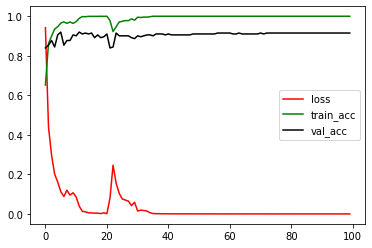
\includegraphics[width=10.5 cm]{img/mlp_train_log.png}
\caption{MLP training history}
\end{figure} 


Classification metrics are on the table.

\begin{specialtable}[H] 
\caption{This is a table caption. Tables should be placed in the main text near to the first time they are~cited.\label{tab1}}

\begin{tabular}{cccc}
\toprule
\textbf{Punch class}	& \textbf{precision}	& \textbf{recall}	& \textbf{F1-score}\\
\midrule
YT		& 0.92		& 0.96		& 0.94\\
MT		& 0.96		& 0.90		& 0.93\\
AT		& 0.93		& 0.85		& 0.89\\
U		& 0.92		& 0.98		& 0.95\\
NP		& 0.85		& 0.87		& 0.86\\
\bottomrule
\end{tabular}
\end{specialtable}

Confusion matrix is on figure

\begin{figure}[H]
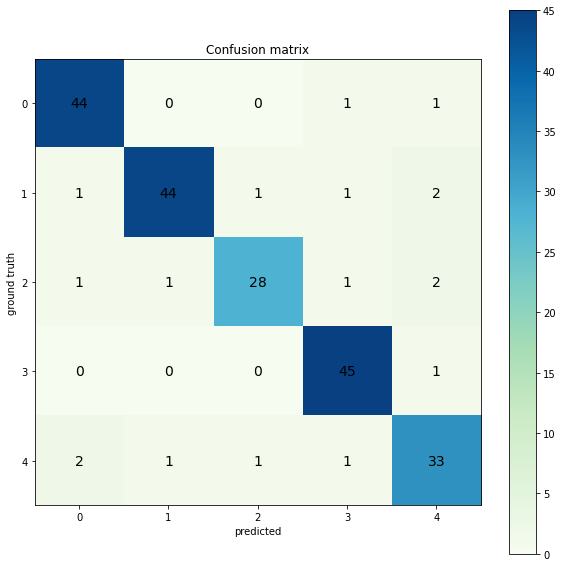
\includegraphics[width=10.5 cm]{img/mlp_confus.png}
\caption{MLP confusion matrix}
\end{figure} 


On training history we see difference between train and validation accuracy and small loss.
This means, that linear model is overfitting.
To avoid this we try more complex model - 1D convolution network.

%%%%%%%%%%%%%%%%%%%%%%%%%%%%%%%%%%%%%%%%%%%%%%%%%%%%%%%%%%%%%%%%%%%%%%%%%%%%%%%%%%%%

\subsection{1D Convolution Net}
1-dimension Convolution Net consist of 3 separate layers with 64 kernels each and relu activations. 
Optimizer is Adam, learning rate = 2e-3 and batch size 64.
100 epochs training history and confusion matrix are on figure.

\begin{figure}[H]
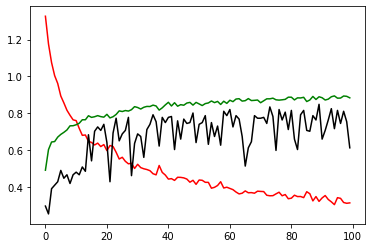
\includegraphics[width=10.5 cm]{img/1conv_train_log.png}
\caption{MLP training history}
\end{figure} 

Classification metrics are on the table 2.

\begin{specialtable}[H] 
\caption{This is a table caption. Tables should be placed in the main text near to the first time they are~cited.\label{tab2}}
\begin{tabular}{cccc}
\toprule
\textbf{Punch class}	& \textbf{precision}	& \textbf{recall}	& \textbf{F1-score}\\
\midrule
YT		& 0.41		& 0.91		& 0.56 \\
MT		& 0.75		& 0.06		& 0.11 \\
AT		& 0.70		& 0.79		& 0.74 \\
U		& 0.91		& 0.63		& 0.74 \\
NP		& 0.83		& 0.79		& 0.81 \\
\bottomrule
\end{tabular}
\end{specialtable}

\begin{figure}[H]
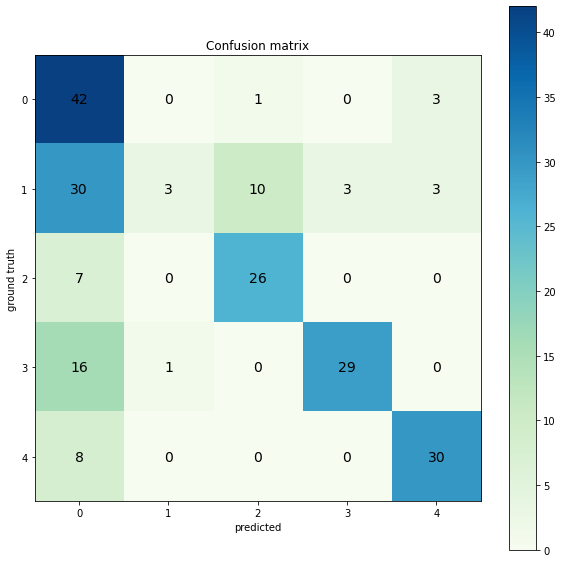
\includegraphics[width=10.5 cm]{img/1conv_confus.png}
\caption{MLP confusion matrix}
\end{figure} 

On training history we see small train accuracy, unstable validation accuracy and big loss.
This means, that 1D conv model is unsuitable for punch classification.
So, we try the model with 2D convolution layers.

%%%%%%%%%%%%%%%%%%%%%%%%%%%%%%%%%%%%%%%%%%%%%%%%%%%%%%%%%%%%%%%%%%%%%%%%%%%%%%%%%%%%

\subsection{2D Convolution Net}
2-dimension Convolution Net consist of 2 layers, that inputs are both x,y and y,z axis. Layers has  72 and 88 kernels, size (2, 52), batch normalization and relu activations. 
Optimizer is Adam, learning rate = 2e-3 and batch size 64.
100 epochs training history and confusion matrix are on figure.

\begin{figure}[H]
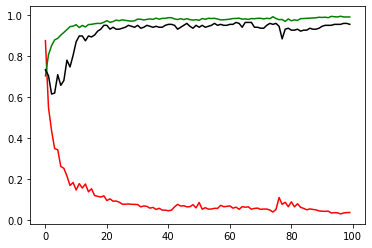
\includegraphics[width=10.5 cm]{img/2conv_train_log.png}
\caption{MLP training history}
\end{figure} 

Classification metrics are on the table 3.

\begin{specialtable}[H] 
\caption{This is a table caption. Tables should be placed in the main text near to the first time they are~cited.\label{tab3}}
\begin{tabular}{cccc}
\toprule
\textbf{Punch class}	&\textbf{precision}	& \textbf{recall}	& \textbf{F1-score}\\
\midrule
YT		& 0.87		& 1.00		& 0.93 \\
MT		& 0.85		& 0.96		& 0.90 \\
AT		& 0.97		& 0.85		& 0.90 \\
U		& 0.95		& 0.85		& 0.90 \\
NP		& 0.97		& 0.87		& 0.92 \\
\bottomrule
\end{tabular}
\end{specialtable}

\begin{figure}[H]
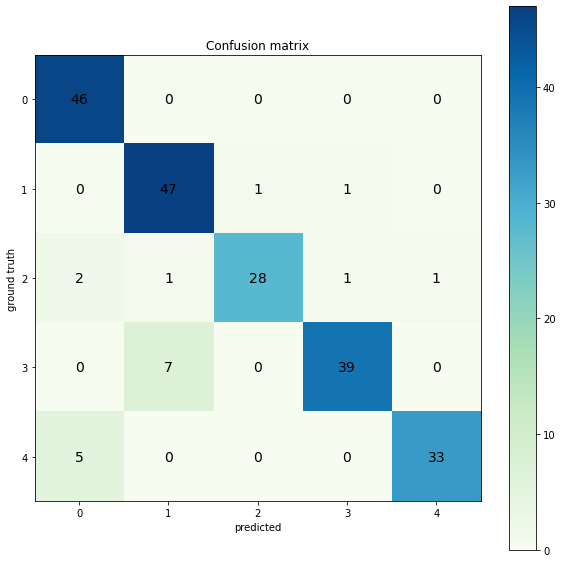
\includegraphics[width=10.5 cm]{img/2conv_confus.png}
\caption{MLP confusion matrix}
\end{figure} 


On training history we see much better train and validation accuracy, small loss.
But can we try deeper model with 4 2D convolution layers?

%%%%%%%%%%%%%%%%%%%%%%%%%%%%%%%%%%%%%%%%%%%%%%%%%%%%%%%%%%%%%%%%%%%%%%%%%%%%%%%%%%%%

\subsection{2D Convolution Net with 4 layers}

2-dimension Convolution Net consist of 2 layers, that inputs are both x,y and y,z axis. Layers has  72 and 88 kernels, size (2, 52), batch normalization and relu activations. 
Optimizer is Adam, learning rate = 2e-3 and batch size 64.
100 epochs training history and confusion matrix are on figure.

\begin{figure}[H]
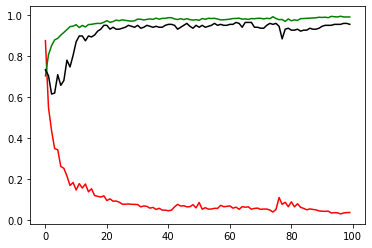
\includegraphics[width=10.5 cm]{img/2conv_train_log.png}
\caption{MLP training history}
\end{figure} 

Classification metrics are on the table 4.
% The MDPI table float is called specialtable
\begin{specialtable}[H] 
\caption{This is a table caption. Tables should be placed in the main text near to the first time they are~cited.\label{tab4}}
%%% \tablesize{} %% You can specify the fontsize here, e.g., \tablesize{\footnotesize}. If commented out \small will be used.
\begin{tabular}{cccc}
\toprule
\textbf{Punch class}	& \textbf{precision}	& \textbf{recall}	& \textbf{F1-score}\\
\midrule
YT		& 0.87		& 1.00		& 0.93 \\
MT		& 0.85		& 0.96		& 0.90 \\
AT		& 0.97		& 0.85		& 0.90 \\
U		& 0.95		& 0.85		& 0.90 \\
NP		& 0.97		& 0.87		& 0.92 \\
\bottomrule
\end{tabular}
\end{specialtable}

\begin{figure}[H]
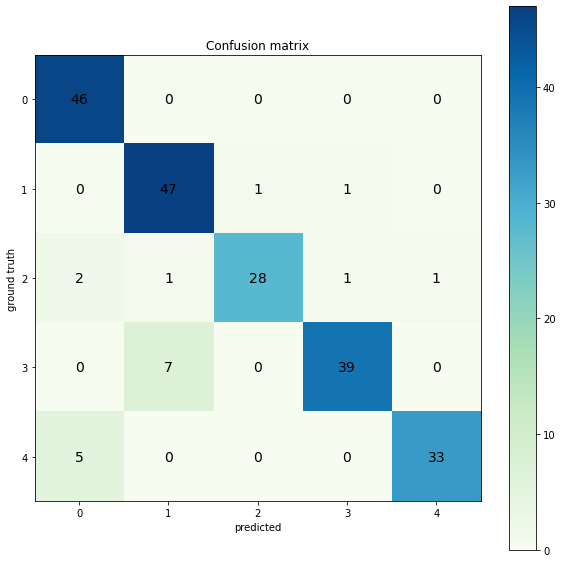
\includegraphics[width=10.5 cm]{img/2conv_confus.png}
\caption{MLP confusion matrix}
\end{figure} 


On training history we see much better train and validation accuracy, small loss.
But can we try deeper model with 4 2D convolution layers?

%%%%%%%%%%%%%%%%%%%%%%%%%%%%%%%%%%%%%%%%%%%%%%%%%%%%%%%%%%%%%%%%%%%%%%%%%%%%%%%%%%%%
\section{Discussion}
Multilayer perceptron is a simple model and good baseline. Best F1 score is 0.95 for U-punch, worst is 0.86 for N-punch. Difference between train and validation accuracy is rusult of model overfiiting.
Increasing number of training samples will solve this problem.\\
1D convolution model from [] work works very bad and not suitable for punch class prediction. Train accuracy is about 0.8, but validation accuracy only 0.65 and very unstable. Worst F1 score is 0.11 for MT-punch, best F1 is 0.81 for No-punch class. Loss after 100 epochs training is only about 0.3.\\
As we proposed, 2D convolution model with 2 conv layers works better. Metrics are like on mlp: best F1 is 0.93 for YT-punch and worst is 0.90 for U-punch class. A little gap between training and validation accuracy curves is tell about some overfitting, so we tested deeper conv model with 4 layers.\\
2D convolution model with 4 conv layer shows best result: 0.97 validation accuracy. Best F1-score 0.99 for YT-punch class, worst 0.90 for AT-punch class.\\
Comparing with MLP, we achieved better classification metrics and shift invariant model, based on 2D convolution. 
\section{Conclusions}
Comparing with classic ML prediction methods, neural nets have a little smaller F1-score, but higher accuracy. 


%%%%%%%%%%%%%%%%%%%%%%%%%%%%%%%%%%%%%%%%%%
\vspace{6pt} 

%%%%%%%%%%%%%%%%%%%%%%%%%%%%%%%%%%%%%%%%%%
%% optional
%\supplementary{The following are available online at \linksupplementary{s1}, Figure S1: title, Table S1: title, Video S1: title.}

% Only for the journal Methods and Protocols:
% If you wish to submit a video article, please do so with any other supplementary material.
% \supplementary{The following are available at \linksupplementary{s1}, Figure S1: title, Table S1: title, Video S1: title. A supporting video article is available at doi: link.} 

%%%%%%%%%%%%%%%%%%%%%%%%%%%%%%%%%%%%%%%%%%
%\authorcontributions{For research articles with several authors, a short paragraph specifying their individual contributions must be provided. The following statements should be used ``Conceptualization, X.X. and Y.Y.; methodology, X.X.; software, X.X.; validation, X.X., Y.Y. and Z.Z.; formal analysis, X.X.; investigation, X.X.; resources, X.X.; data curation, X.X.; writing---original draft preparation, X.X.; writing---review and editing, X.X.; visualization, X.X.; supervision, X.X.; project administration, X.X.; funding acquisition, Y.Y. All authors have read and agreed to the published version of the manuscript.'', please turn to the  \href{http://img.mdpi.org/data/contributor-role-instruction.pdf}{CRediT taxonomy} for the term explanation. Authorship must be limited to those who have contributed substantially to the work~reported.}

\funding{This research received no external funding.}

\institutionalreview{The study was conducted according to the guidelines of the Declaration of Helsinki, and approved by the Institutional Review Board (or Ethics Committee) of Financial University under the Government of the Russian Federation.}

\informedconsent{Informed consent was obtained from all subjects involved in the study.}

%\dataavailability{In this section, please provide details regarding where data supporting reported results can be found, including links to publicly archived datasets analyzed or generated during the study. Please refer to suggested Data Availability Statements in section ``MDPI Research Data Policies'' at \url{https://www.mdpi.com/ethics}. You might choose to exclude this statement if the study did not report any data.} 

\acknowledgments{The author would like to thank athletes, coaches, and the leadership of the
Karate Federation of the Republic of Tatarstan (Kazan, Russia) for organizing the experiments and
actively participating in the study.}

\conflictsofinterest{The authors declare no conflict of interest.} 

%% Optional
%\sampleavailability{Samples of the compounds ... are available from the authors.}

%%%%%%%%%%%%%%%%%%%%%%%%%%%%%%%%%%%%%%%%%%
%% Only for journal Encyclopedia
%\entrylink{The Link to this entry published on the encyclopedia platform.}

%%%%%%%%%%%%%%%%%%%%%%%%%%%%%%%%%%%%%%%%%%
%% Optional
\abbreviations{The following abbreviations are used in this manuscript:\\

\noindent 
\begin{tabular}{@{}ll}
MDPI & Multidisciplinary Digital Publishing Institute\\
DOAJ & Directory of open access journals\\
TLA & Three letter acronym\\
LD & Linear dichroism
\end{tabular}}

%%%%%%%%%%%%%%%%%%%%%%%%%%%%%%%%%%%%%%%%%%
%% Optional
\appendixtitles{no} % Leave argument "no" if all appendix headings stay EMPTY (then no dot is printed after "Appendix A"). If the appendix sections contain a heading then change the argument to "yes".
\appendixstart
\appendix

%%%%%%%%%%%%%%%%%%%%%%%%%%%%%%%%%%%%%%%%%%
\reftitle{References}

% Please provide either the correct journal abbreviation (e.g. according to the “List of Title Word Abbreviations” http://www.issn.org/services/online-services/access-to-the-ltwa/) or the full name of the journal.
% Citations and References in Supplementary files are permitted provided that they also appear in the reference list here. 

%=====================================
% References, variant A: external bibliography
%=====================================
%\externalbibliography{yes}
%\bibliography{your_external_BibTeX_file}

%=====================================
% References, variant B: internal bibliography
%=====================================
\begin{thebibliography}{999}

\bibitem[Polak(2016)]{ref-journal1}
Polak, E.; Kulasa, J.; VencesBrito, A.; Castro, M.; Fernandes, O. Motion analysis systems as optimization training tools in combat sports and martial arts. {\em Revista de Artes Marciales Asiáticas} {\bf 2016}, {\em 10(2)}, 105-123. doi:http://dx.doi.org/10.18002/rama.v10i2.1687

\bibitem[Worsey(2019)]{ref-journal2}
Worsey, M.T.; Espinosa, H.G.; Shepherd, J.B.; Thiel, D.V. Inertial Sensors for Performance Analysis in Combat Sports: A Systematic Review. {\em Sports (Basel)} {\bf 2019}, {\em 7(1)} 28. doi:10.3390/sports7010028

\bibitem[Kimm(2015)]{ref-journal3}
Kimm, D.; K.; Thiel, D. Hand Speed Measurements in Boxing. {\em Procedia Engineering}, {\bf 2015}, {\em Volume 112}, 502-506. https://doi.org/10.1016/j.proeng.2015.07.232

\bibitem[Dinu(2020)]{ref-journal4}
Dinu, D.; Millot, B.; Slawinski, J.; Louis, J. An Examination of the Biomechanics of the Cross, Hook and Uppercut between Two Elite Boxing Groups. {\em Proceedings} {\bf 2020}, {\em 49}, 61. https://doi.org/10.3390/proceedings2020049061

\bibitem[Haralabidis(2020)]{ref-journal5}
Haralabidis, N.; Saxby, D.J.; Pizzolato, C.; Needham, L.; Cazzola, D.; Minahan, C. Fusing Accelerometry with Videography to Monitor the Effect of Fatigue on Punching Performance in Elite Boxers. {\em Sensors} {\bf 2020}, {\em 20}, 5749. https://doi.org/10.3390/s20205749

\bibitem[Cust(2019)]{ref-journal6}
Cust, E. E.; Sweeting, A. J.; Ball, K.; Robertson, S. Machine and deep learning for sport-specific movement recognition: a systematic review of model development and performance. {\em Journal of sports sciences}, {\bf 2019}, {\em 37(5)}, 568–600. https://doi.org/10.1080/02640414.2018.1521769

\bibitem[Khasanshin(2021)]{ref-journal7}
Khasanshin, I. Application of an Artificial Neural Network to Automate the Measurement of Kinematic Characteristics of Punches in Boxing. {\em Appl. Sci}. {\bf 2021}, {\em 11}, 1223. https://doi.org/10.3390/app11031223

\bibitem[Worsey(2020)]{ref-journal8}
Worsey, M.T.O.; Espinosa, H.G.; Shepherd, J.B.; Thiel, D.V. An Evaluation of Wearable Inertial Sensor Configuration and Supervised Machine Learning Models for Automatic Punch Classification in Boxing. {\em IoT} {\bf 2020}, {\em 1}, 360–381, doi:10.3390/iot1020021.

\end{thebibliography}

%%%%%%%%%%%%%%%%%%%%%%%%%%%%%%%%%%%%%%%%%%
%% for journal Sci
%\reviewreports{\\
%Reviewer 1 comments and authors’ response\\
%Reviewer 2 comments and authors’ response\\
%Reviewer 3 comments and authors’ response
%}
%%%%%%%%%%%%%%%%%%%%%%%%%%%%%%%%%%%%%%%%%%
\end{document}